%
% report.tex - tex model of graduation work
% Version 0.1
%
% Author: Paulo S. Machado
% Date: 2S 2011
%
% Release under de GNU Public License v3.0 or greater
% This library is free software; you can redistribute it and/or
% modify it under the terms of the GNU General Public
% License as published by the Free Software Foundation; either
% version 3.0 of the License, or (at your option) any later version.
% 
% This template is distributed in the hope that it will be useful,
% but WITHOUT ANY WARRANTY; without even the implied warranty of
% MERCHANTABILITY or FITNESS FOR A PARTICULAR PURPOSE.  See the GNU
% General Public License for more details.
% 
% You should have received a copy of the GNU Lesser General Public
% License along with this template; if not, write to the Free Software
% Foundation, Inc., 51 Franklin St, Fifth Floor, Boston, MA  02110-1301  USA
%
\documentclass[a4paper,11pt]{article}

%
% preamble.tex - tex model of graduation work
% Version 0.1
%
% Author: Paulo S. Machado
% Date: June 2010
%
% Release under de GNU Public License v3.0 or greater
% This library is free software; you can redistribute it and/or
% modify it under the terms of the GNU General Public
% License as published by the Free Software Foundation; either
% version 3.0 of the License, or (at your option) any later version.
% 
% This template is distributed in the hope that it will be useful,
% but WITHOUT ANY WARRANTY; without even the implied warranty of
% MERCHANTABILITY or FITNESS FOR A PARTICULAR PURPOSE.  See the GNU
% General Public License for more details.
% 
% You should have received a copy of the GNU Lesser General Public
% License along with this template; if not, write to the Free Software
% Foundation, Inc., 51 Franklin St, Fifth Floor, Boston, MA  02110-1301  USA
%
% Language
\usepackage[portuges,brazil]{babel}
\usepackage[top=3cm,bottom=3cm,left=3.0cm,right=3cm]{geometry}
\usepackage[pdftex]{graphicx}
\usepackage{listings}
\usepackage{textcomp}
\usepackage{amssymb}
\usepackage{amsmath}
\usepackage{color}
% Encoding
\usepackage[utf8]{inputenc}

%\usepackage{wrapfig}
%\usepackage{hyperref}

% This will commands into the pdf to create a linked table of contents, as well
%as links for 
% the cross-references such as calls to figure and page numbers 
\usepackage[pagebackref=true]{hyperref}  
\hypersetup{
  pdftitle     = Trabalho de Graduação,
  pdfauthor    = Paulo Silveira Machado,
  colorlinks   = true,
  linkcolor    = black,
  anchorcolor  = red,
  citecolor    = blue,
  filecolor    = red,  
  urlcolor     = red
}



\DeclareGraphicsExtensions{.jpg,.jpeg,.png}
\graphicspath{{../../imagens/}}
% Heading foot
\usepackage{fancyhdr}
\pagestyle{fancy}
\headheight 15pt
\renewcommand{\sectionmark}[1]{\markright{\thesection\ #1}}
\rhead[\fancyplain{}{\bfseries\thepage}] %
    {\fancyplain{}{\bfseries\rightmark}}
\lhead{}
%\lhead[\fancyplain{}{\scshape\leftmark}] %
%    {\fancyplain{}{\bfseries\thepage}}
\cfoot{--~\thepage~--}

\parindent 1cm

% \parskip 5pt

\begin{document}

% Title page and table of contents
%
% title.tex - tex model of graduation work
% Version 0.1
%
% Author: Paulo S. Machado
% Date: June 2010
%
% Release under de GNU Public License v3.0 or greater
% This library is free software; you can redistribute it and/or
% modify it under the terms of the GNU General Public
% License as published by the Free Software Foundation; either
% version 3.0 of the License, or (at your option) any later version.
% 
% This template is distributed in the hope that it will be useful,
% but WITHOUT ANY WARRANTY; without even the implied warranty of
% MERCHANTABILITY or FITNESS FOR A PARTICULAR PURPOSE.  See the GNU
% General Public License for more details.
% 
% You should have received a copy of the GNU Lesser General Public
% License along with this template; if not, write to the Free Software
% Foundation, Inc., 51 Franklin St, Fifth Floor, Boston, MA  02110-1301  USA
%
% Title page
\begin{titlepage}
\begin{center}
 
% Header

\includegraphics[width=0.15\textwidth]{figures/unicamp128}\\[1cm]
\textsc{\LARGE Universidade Estadual de Campinas}\\[0.3cm]
\textsc{\LARGE ES952 - Trabalho de Graduação II}\\[3.0cm] 
\textsc{\Large Relatório de Atividades} \\[0.2cm]

  
% Title
\hfill
\textsf{ \LARGE \bfseries Desenvolvimento de um câmbio automático para
bicicletas}

\vfill
% Author and project
\begin{minipage}{0.49\textwidth}
\begin{flushleft} \large
\emph{Autor:}\\
Paulo Silveira Machado \\
RA: 024831
\end{flushleft}
\end{minipage}
\begin{minipage}{0.5\textwidth}
\begin{flushright} \large
\emph{Orientador:} \\
Prof. Dr. Luiz Otávio Saraiva Ferreira\\
Faculdade de Engenharia Mecânica
\end{flushright}
\end{minipage}
 
\vfill
 
% Botton
{\large 2\textordmasculine ~Semestre/2011}
\end{center}
 
\end{titlepage}

% Table of contents
\tableofcontents
\pagebreak

% List of figures
\listoffigures
\pagebreak

% List of tables
\listoftables
\pagebreak

\lstset{frame=single,
    showstringspaces=false,
    extendedchars=true,
    language=C++,
    backgroundcolor=\color[rgb]{0.95,0.95,0.95},
    rulecolor=\color[rgb]{0.3,0.3,0.3},
    basicstyle=\scriptsize\ttfamily,
    commentstyle=\color[RGB]{105,105,105}\rmfamily\itshape,
    keywordstyle=\color[rgb]{0.6,0.0,0.0}\bfseries,
    stringstyle=\color[rgb]{0.6,0.4,0.4},
    identifierstyle=\color[rgb]{0.0,0.0,0.5},
    basicstyle=\tiny,
}

%%%
%
\section{Resumo}
\label{sec:resumo}
Um trabalho de graduação em Engenharia de Controle e Automação deve,
idealmente, abranger as três grandes áreas que originam essa
formação\cite{enciclo}: Engenharia Elétrica (eletrônica, processamento de
sinais, circuitos elétricos e teoria de controle, etc); Engenharia
Mecânica (dinâmica, modelagem de sistemas, etc); e a Computação (automação,
controle discreto, etc). Este trabalho tenta, modestamente, resvelar por cada
uma destas áreas e honrar a formação recebida.

A ideia deste projeto surgiu das observações diárias de ciclistas e do
uso da bicicleta, onde grande parte das pessoas não sabe utilizar de
forma eficiente as marchas de suas bicicletas. Estas parecem ser
complicadas (\textit{mountain bikes} simples possuem pelo menos 18 marchas) e de
difícil manejo e configuração. Assim como em uma transmissão automotiva, maus
hábitos no seu manejo -- esticar marchas, manter a mão apoiada sobre a alavanca,
entre outros -- causam desgaste precoce dos componentes, esforços desnecessários
(neste caso para ciclista) e até risco de segurança.

O benefício primordial de qualquer automação (i.e. retirar do usuário o
controle ou parte do controle sobre o sistema que interage) é a melhora no
fluxo do processo devido ao grande controle que tem se sobre o sistema. Os
resultados deste benefício são, em alto nível, o aumento da qualidade,
repetibilidade e uniformidade, aplicação de estratégias ótimas de controle e
simplicidade na interação com utilizador.

Este relatório apresenta o desenvolvimento e resultados do trabalho proposto e
estudado na primeira disciplina de Trabalho de Graduação: a construção de um
protótipo funcional de um sistema de troca de marchas automatizados para
bicicletas convencionais. Neste primeiro trabalho foram construídas as base
teóricas e ferramentais para a construção de um protótipo funcional: construção
da bancada experimental; desenvolvimento da lógica; e estudo de soluções 
existentes. Ou seja, dados os objetivos do projeto -- software de controle,
circuito de controle, atuados mecânico e a junção destes no protótipo --
apresenta-se o caminho percorrido até o objetivo e os resultados alcançados.

O documento foi estruturado de forma a descrever o problema de engenharia, as
alternativas consideradas, escolhas e desenvolvimento de cada parte funcional do
protótipo final.


\pagebreak
%%%
%
\section{Introdução}
\label{sec:intro}
Automação ou Controle? Esta foi a tônica no início do desenvolvimento
deste projeto. A solução de controle é mais elegante, porém seu desenvolvimento
é mais complexo e depende de um sinal contínuo. A automação não é tão elegante e
eficiente, porém seu desenvolvimento é mais simples e pode ser orientada a
eventos. A resposta, seja ela qual for, passa obrigatoriamente pela análise do
problema físico.

\subsection{Análise do problema físico}
A transmissão ciclística é tal qual mostrado na figura \ref{fig:transmissao}.
\begin{figure}[ht]
\begin{center}
 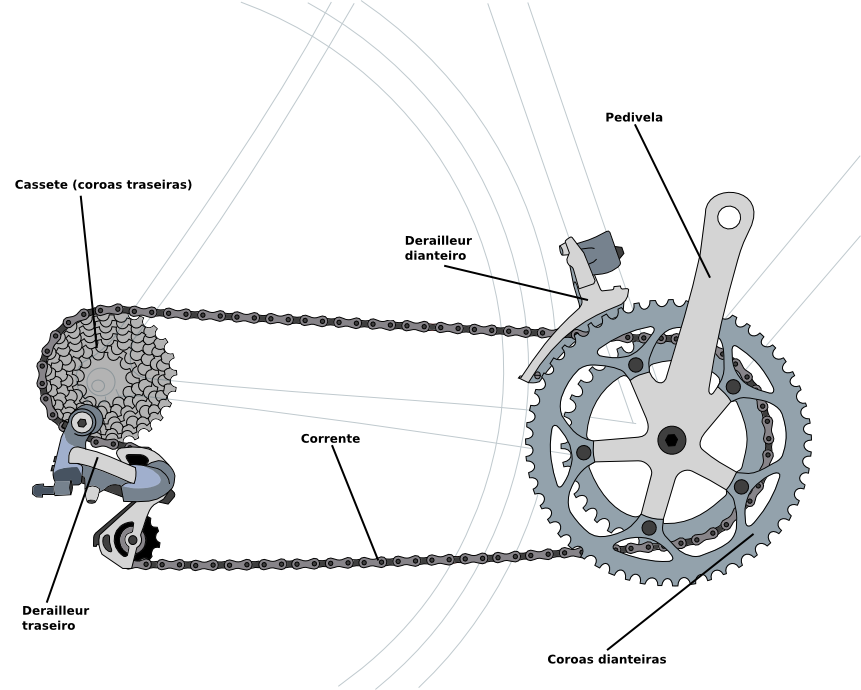
\includegraphics[width=5.5in]{transmissao}
\end{center}
  \caption{Componentes de uma transmissão ciclística}
  \label{fig:transmissao}
\end{figure}
Podemos observar os principais componentes da transmissão, sendo na ordem em que
a energia é transmitida: o pedivela transmite o torque aplicado aos pedais pelo
ciclista às coroas dianteiras, que movimentam a corrente, que por sua vez,
transmite a energia às coroas traseiras (o conjunto destas é chamado de cassete,
nome que será usado no documento), conectadas a roda traseira, gerando a
movimento.

A relação de transmissão é determinada pela quantidade de dentes da coroa
traseira e dianteira de um engrenamento. Assim, a troca de marcha
(i.e. da relação de transmissão) é realizada pela mudança no engrenamento da
corrente com as coroas, tanto dianteiras  quanto traseiras. Portanto uma
bicicleta possui tantas marchas quanto forem a multiplicação da quantidade de
coroas no cassete pelas coroas dianteiras, por exemplo, quando há três coroas
dianteiras e seis coroas no cassete, a transmissão possui 3x6=18 marchas.
A mudança no engrenamento é realizado pelos
\textit{derailleurs}\footnote{\textit{Derailleur} é um termo francês que pode
ser traduzido como o ato do descarrilamento de um trem na ferrovia. O
dispositivo ganhou esse nome devido à semelhança com o evento.}, que mediante ao
deslocamento longitudinal ao eixo da roda força a corrente ser engrenada em
outra coroa.

O desenvolvimento do protótipo é tratado como uma prova de conceito, e por
simplicidade, a atuação vai ser concentrada nos componentes da parte traseira
da transmissão, ou seja, no \textit{derailleur}.
O esquema da figura \ref{fig:derailleur} apresenta a visão traseira
do \textit{derailleur} traseiro e três exemplos de engrenamento.
\begin{figure}[ht]
\begin{center}
 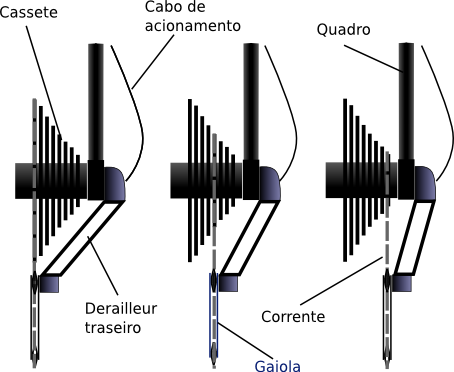
\includegraphics[width=4in]{derailleur}
\end{center}
  \caption{Três engrenamentos}
  \label{fig:derailleur}
\end{figure}
Na figura \ref{fig:derailleur} temos, respectivamente, engrenado uma marcha
lenta (alto torque e baixa velocidade), uma marcha média e uma marcha rápida
(baixo torque e alta velocidade). O movimento da gaiola (componente do
\textit{derailleur}) se dá pela sua estrutura de braços paralelos do
\textit{derailleur} e é acionado via cabo, com retorno por mola. O cabo é
controlado pelo ciclista, geralmente por um sistema alavanca montado no guidão,
mas que também assume diversas outras formas, sempre com o objetivo de puxar ou
soltar o cabo, e genericamente chamado trocador (\textit{shifter}). O
trocador movimenta o cabo em estágios discretos, sendo cada estágio desse
correspondente ao engrenamento em uma coroa diferente.

O ciclista controla a pedalada de acordo com seu gosto, terreno e
velocidade. Logo, quando está em um aclive, procura puxar o cabo de forma a
engrenar as marchas mais lentas, e o oposto quando enfrenta um declive ou um
terreno que ofereça menos resistência, como por exemplo asfalto plano. O gosto e
biótipo do ciclista determinam o ponto da troca de marcha pela velocidade da
cadência (velocidade da pedalada). Por exemplo, o sete vezes campeão do
\textit{Tour de France}, Lance Armstrong, prefere pedalar em alta velocidade
(picos de 100-110 RPM), enquanto que outros ciclistas de sua categoria
dificilmente alcançam 90 RPM de
cadência\footnote{
www.trifuel.com/training/bike/cycling-cadence-and-pedaling-economy}.
Ciclistas amadores possuem limites bem inferiores. Portanto, uma premissa básica
do projeto é a possibilidade do ajuste sobre os limites para a troca de marcha.

O resultado da análise do problema físico levou a escolha pela solução de
automação, preterindo o controle. A decisão baseou-se na observação de que o
sistema de uma transmissão de bicicleta, considerando as possíveis alternativas
para a forma de aquisição de dados de custo acessível, é orientado a
eventos e baseado em estados discretos.

\subsection{Revisão bibliográfica}
Uma ampla revisão bibliográfica foi realizada na primeira parte deste Trabalho
de Graduação, e não será repetida neste relatório. Vale ressaltar porém, que
pouca bibliografia acadêmica é produzida sobre o assunto. Por outro lado, o
desenvolvimento comercial é bastante prolífico, havendo em torno de quatro ou
cinco companhias multinacionais liderando os mercados globais de componentes e
diversos garagistas pensando e desenvolvendo soluções.

O problema que surge é como localizar documentação sobre uma solução tão
específica? A resposta foi a utilização de duas bases de patentes:
USPTO\cite{uspto} e EPO\cite{epo}. O critério de escolha utilizado para
selecionar apenas os dois escritórios foi o fato de constituírem os dois maiores
mercados consumidores do mundo.


\subsection{Premissas do projeto}
Após o estabelecimento do tipo de solução e de alguns requisitos mínimos, as
premissas estabelecidas para o projeto são:
\begin{itemize*}
  \item Baixo custo
  \item Adaptabilidade ao sistema existente
  \item Possibilidade de configuração de parâmetros
  \item Interface com usuário
\end{itemize*}



\pagebreak
%%%
%
\section{Desenvolvimento das partes}
\label{sec:partes}
Nesta seção são apresentadas as partes do projeto e como estas foram unidas. O
desenvolvimento deste projeto foi modular, o que permitiu na maior parte do
tempo trabalhar no hardware e no software de forma independente. As partes são:
\begin{itemize*}
  \item Bancada experimental
  \item Circuito de controle
  \item Protótipo Completo
  \item Algoritmo de Controle
\end{itemize*}


\subsection{Bancada experimental}
\label{sec:bancada}
A bancada experimental é um dos produtos principais da primeira parte deste
trabalho de graduação. Simular os sinais do sistema via algum tipo de software
ou kit é uma opção menos desejável, visto que o de desenvolvimento
do projeto com base em um sistema real não se apresentou como uma proposta
complicada ou muito cara. Desta forma, a solução elaborada no primeiro trabalho
foi usar uma bicicleta convencional e adaptá-la de forma a criar uma bancada de
testes. O resultado é apresentado na Figura
\ref{fig:bancada}.
\begin{figure}[ht]
 \begin{center}
  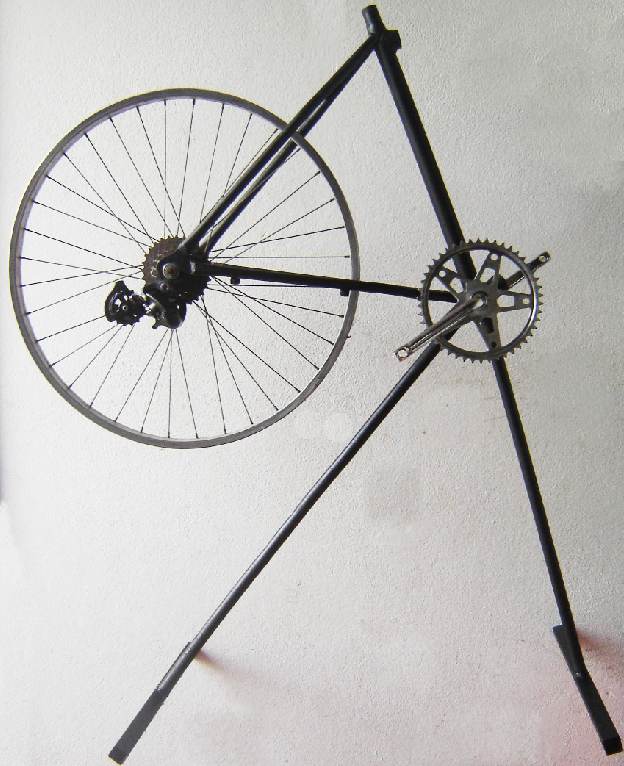
\includegraphics[width=3.5in]{bancada_tratada}
 \end{center}
 \caption{Bancada experimental construída para o TG I}
 \label{fig:bancada}
\end{figure}
A bancada é uma meia bicicleta -- com a parte traseira, onde estão os
elementos da transmissão  -- onde foram soldados apoios, possibilitando
``pedalar no vazio'' e realizar os testes do projeto em um sistema real.

Foram diversos os problemas relativos a bancada, e surgiram no momento prévio
aos testes, quando os componentes da transmissão foram montados. As peças
disponíveis não eram compatíveis (corrente curta, coroa dianteira
não casou com o corrente), o que causou novos custos e atraso nos testes.
Superados os percalços, o resultado final é apresentado na figura
\ref{fig:setup}. Nesta montagem estão presentes, além do sistema mecânico
completo da bicicleta, a montagem do servo motor e os ímas acoplados ao
pedivela e a roda.
\begin{figure}[h!]
\begin{center}
 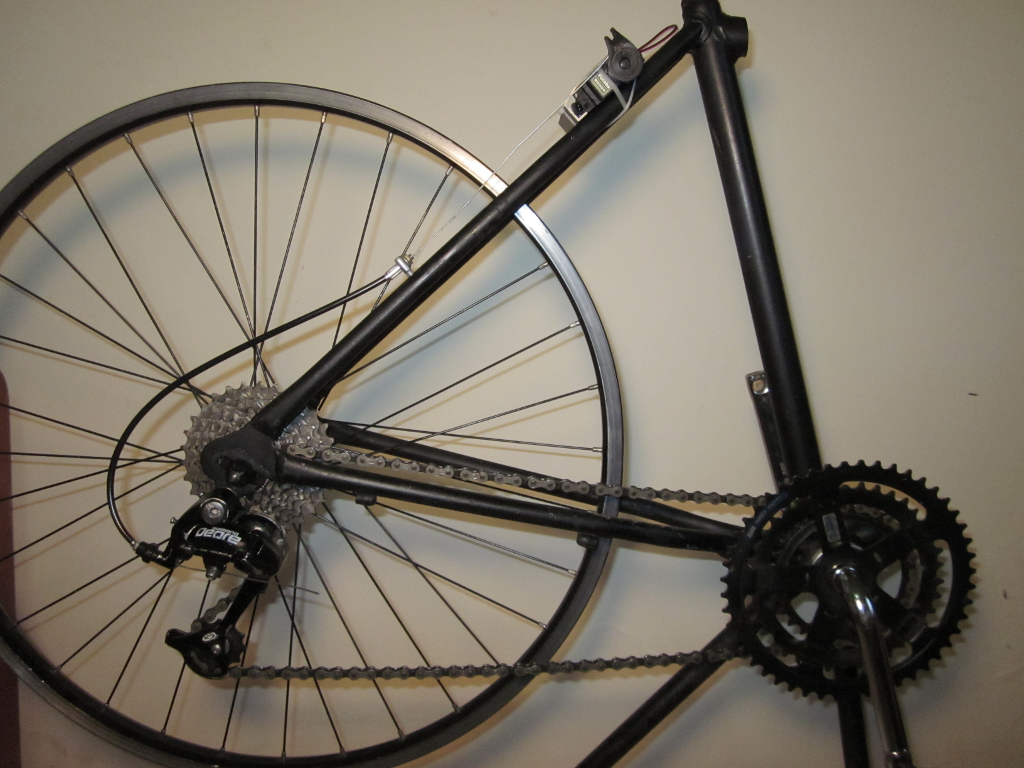
\includegraphics[width=5in]{setup}
\end{center}
  \caption{Bancada pronta para teste}
  \label{fig:setup}
\end{figure}


%%%
%
\subsection{Circuito de controle}
\label{sec:montagem}
O circuito de controle foi montado sobre uma placa de prototipação (protoboard)
e seu esquema geral é apresentado na figura \ref{fig:montagem}.
Os componentes podem ser separados em três grupos funcionais: saídas, controle
e entradas.
\begin{figure}[ht]
\begin{center}
 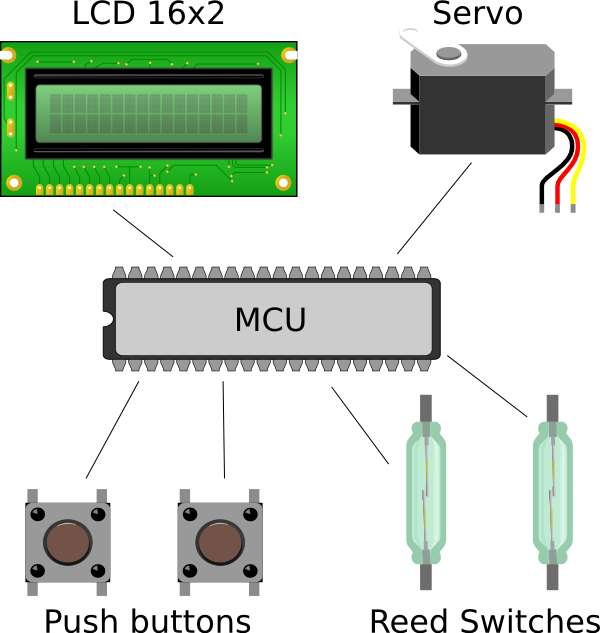
\includegraphics[width=3.2in]{montagem}
\end{center}
  \caption{Componentes da montagem do circuito de controle}
  \label{fig:montagem}
\end{figure}
Nessa classificação são: saídas, servo motor e LCD (\textit{Liquid
Crystal Display}; controle, MCU (\textit{MicroControler Unit}); e entradas os
\textit{push buttons} e \textit{reed switch}. Os componentes utilizados e
detalhes da integração são descritos a seguir.

\subsubsection{Servo Motor}
\label{sec:servo}
O servo motor é o único atuador deste projeto, sendo responsável pela atuação
sobre o cabo do \textit{derailleur} e consequente troca de marchas. Duas
perguntas foram elaboradas para ajudar na definição de um atuador: Qual a
forma mais simples de atuar sobre um cabo utilizando um motor rotativo? Qual
tipo de motor é confiável de controle simples? A reposta, encontrada a partir
do estudo realizado na primeira parte do trabalho de graduação é, uma polia
acoplada a um servo motor.

O raio da polia foi dimensionado de tal forma que, dado que um servo motor
rotaciona 180\textdegree, meia circunferência da polia seja deslocamento
suficiente para movimentar o \textit{derailleur} da menor a maior marcha.
Assim, definimos o raio da polia ($r_{polia}$), o número de marchas (n) e o
passo (p) como o deslocamento necessário do cabo de comando para a mudança de
uma marcha consecutiva, de tal forma que:
\begin{equation*}
  \frac{\displaystyle 2\pi r_{polia} }{\displaystyle 2} = (n-1)p
\end{equation*}
\begin{equation}
  r_{polia} = \frac{\displaystyle (n-1)p}{\displaystyle \pi}
\end{equation}
Para a bancada de testes, n=6 e p=3 mm. O raio ideal para a polia é:
\begin{equation}
 r_{polia} = \frac{\displaystyle (6-1)\times 3}{\displaystyle \pi} = 4.77~mm
\end{equation}
Porém, este resultado não foi utilizado, pois a construção de uma polia foi
preterida pela adaptação de um trocador manual (figura \ref{fig:shifter}).
\begin{figure}[h!]
\begin{center}
 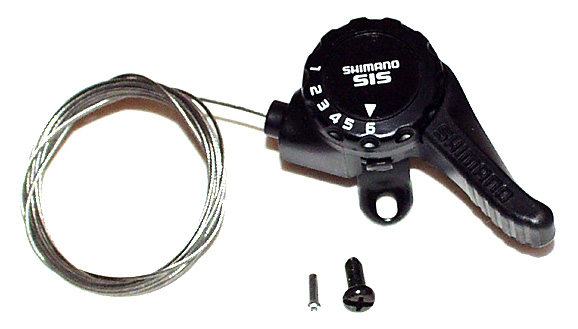
\includegraphics[width=4in]{shifter}
\end{center}
  \caption{Trocador manual antes da adaptação}
  \label{fig:shifter}
\end{figure}

A polia interna deste trocador possui raio de 8.5 mm, o que por um lado aumenta
o intervalo de marchas disponível e a velocidade da troca, por outro aumenta o
requisito de torque no eixo. A figura \ref{fig:atuador} mostram a sequência da
adaptação.
\begin{figure}[h!]
 \centering
  \subfloat[Partes]{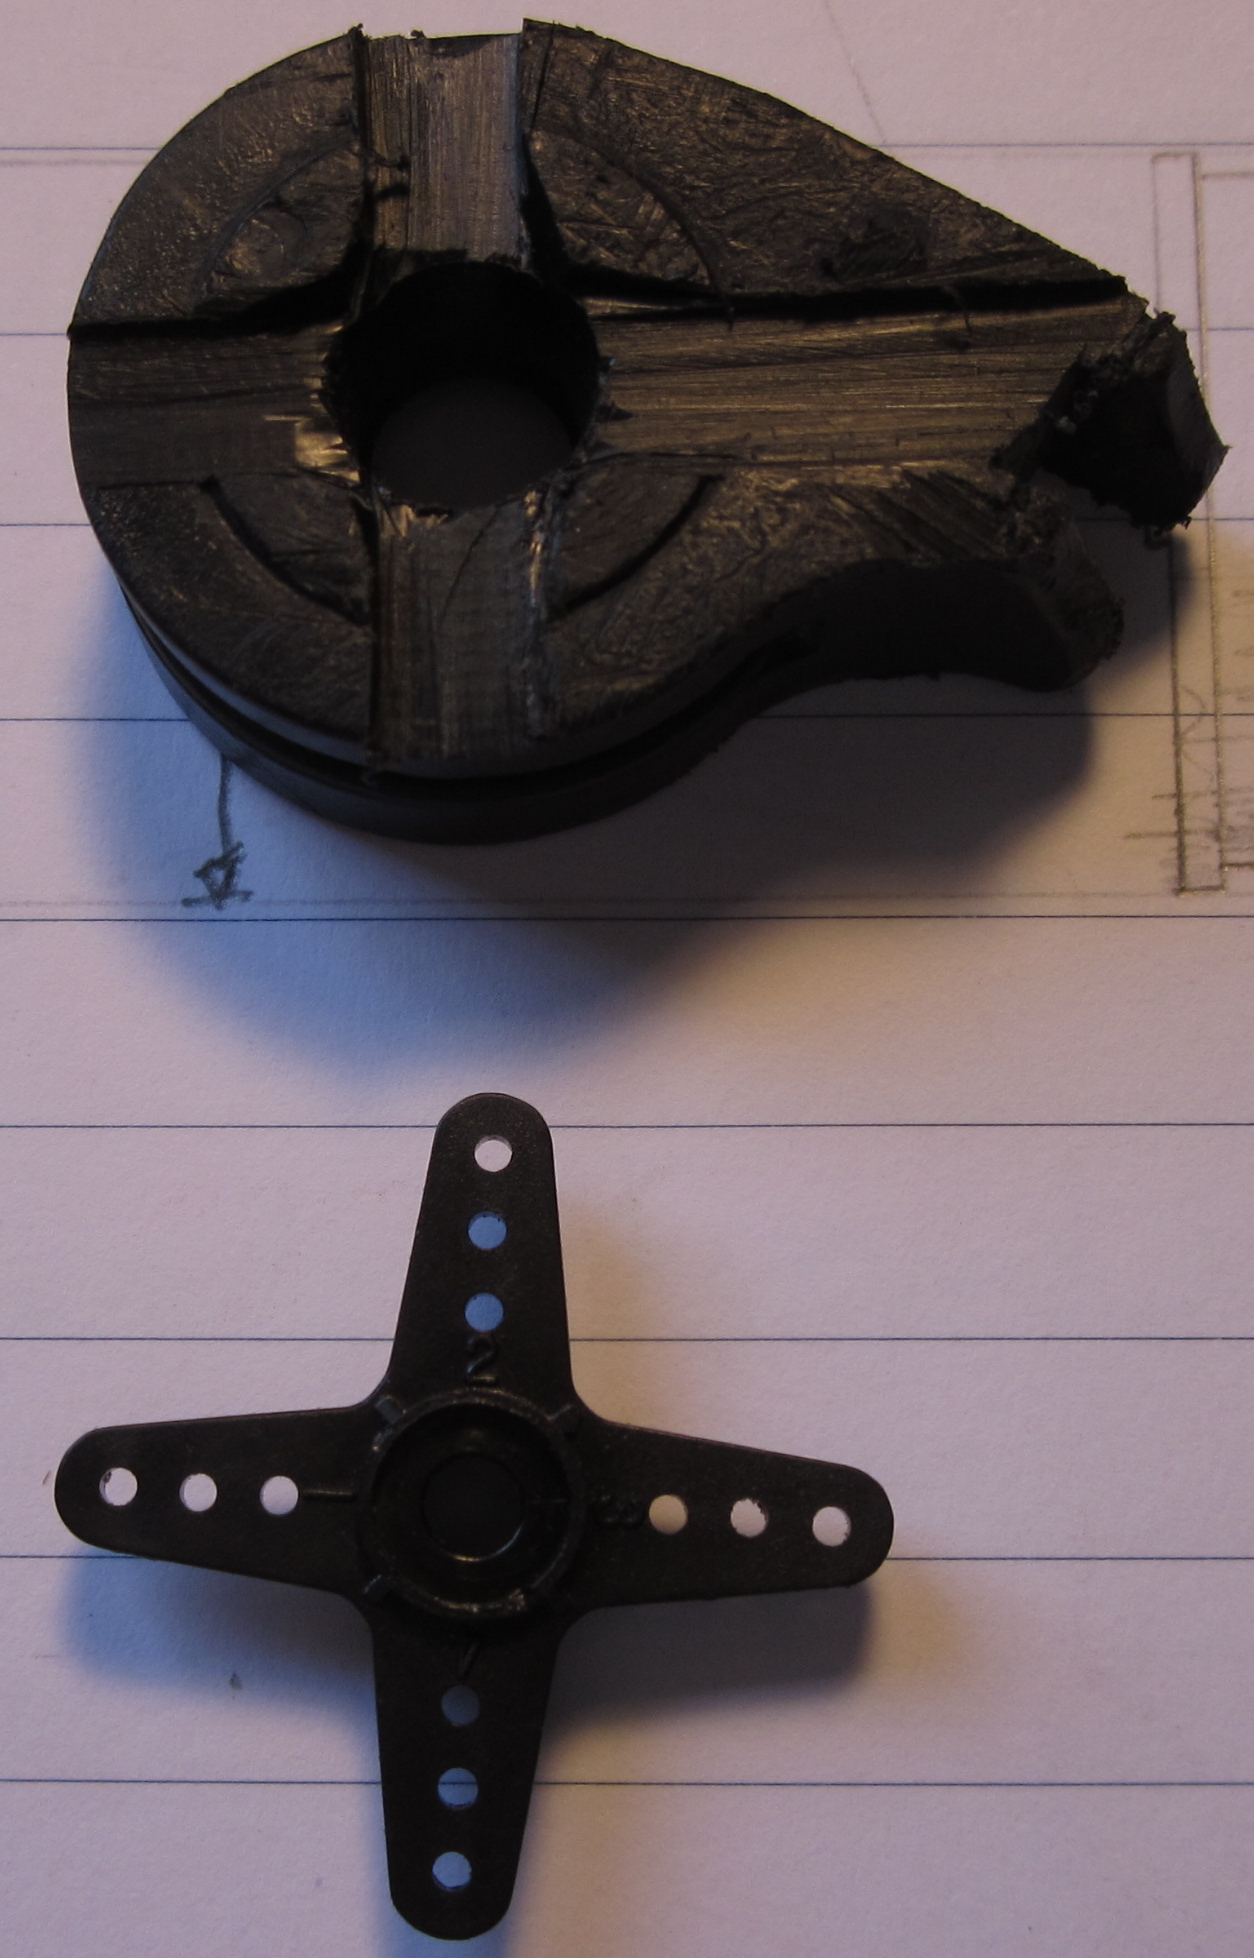
\includegraphics[width=1.9in]{polia1}} \hfil
  \subfloat[Partes Montadas]{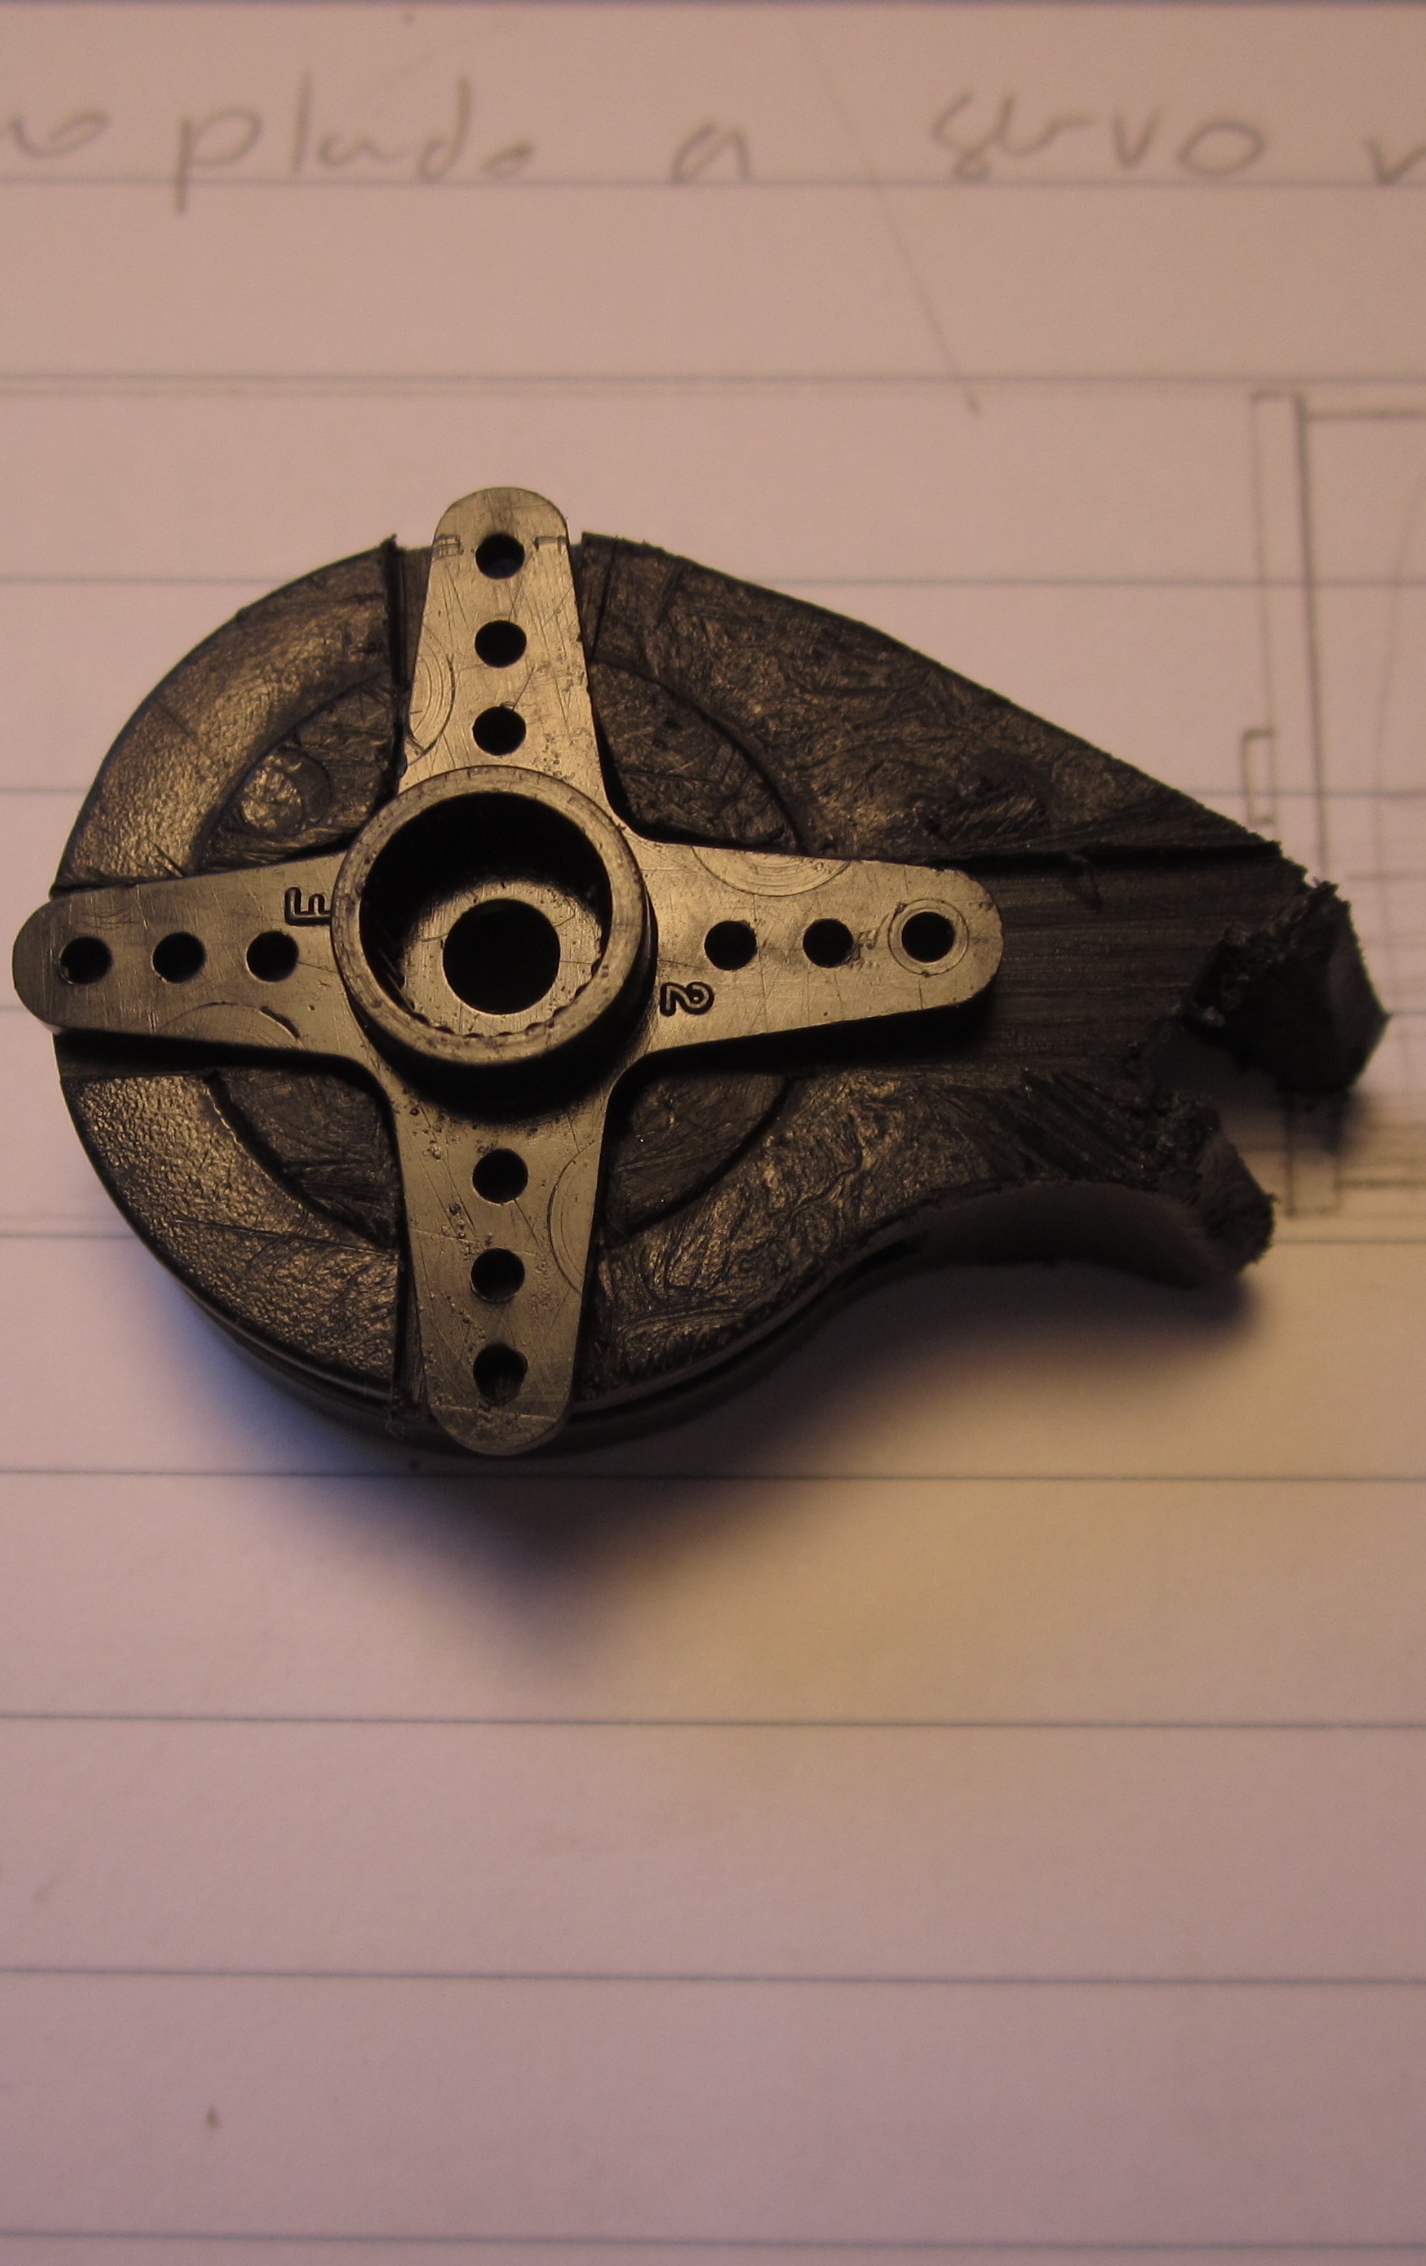
\includegraphics[width=1.87in]{polia2}} \hfil
  \subfloat[Atuador Completo]{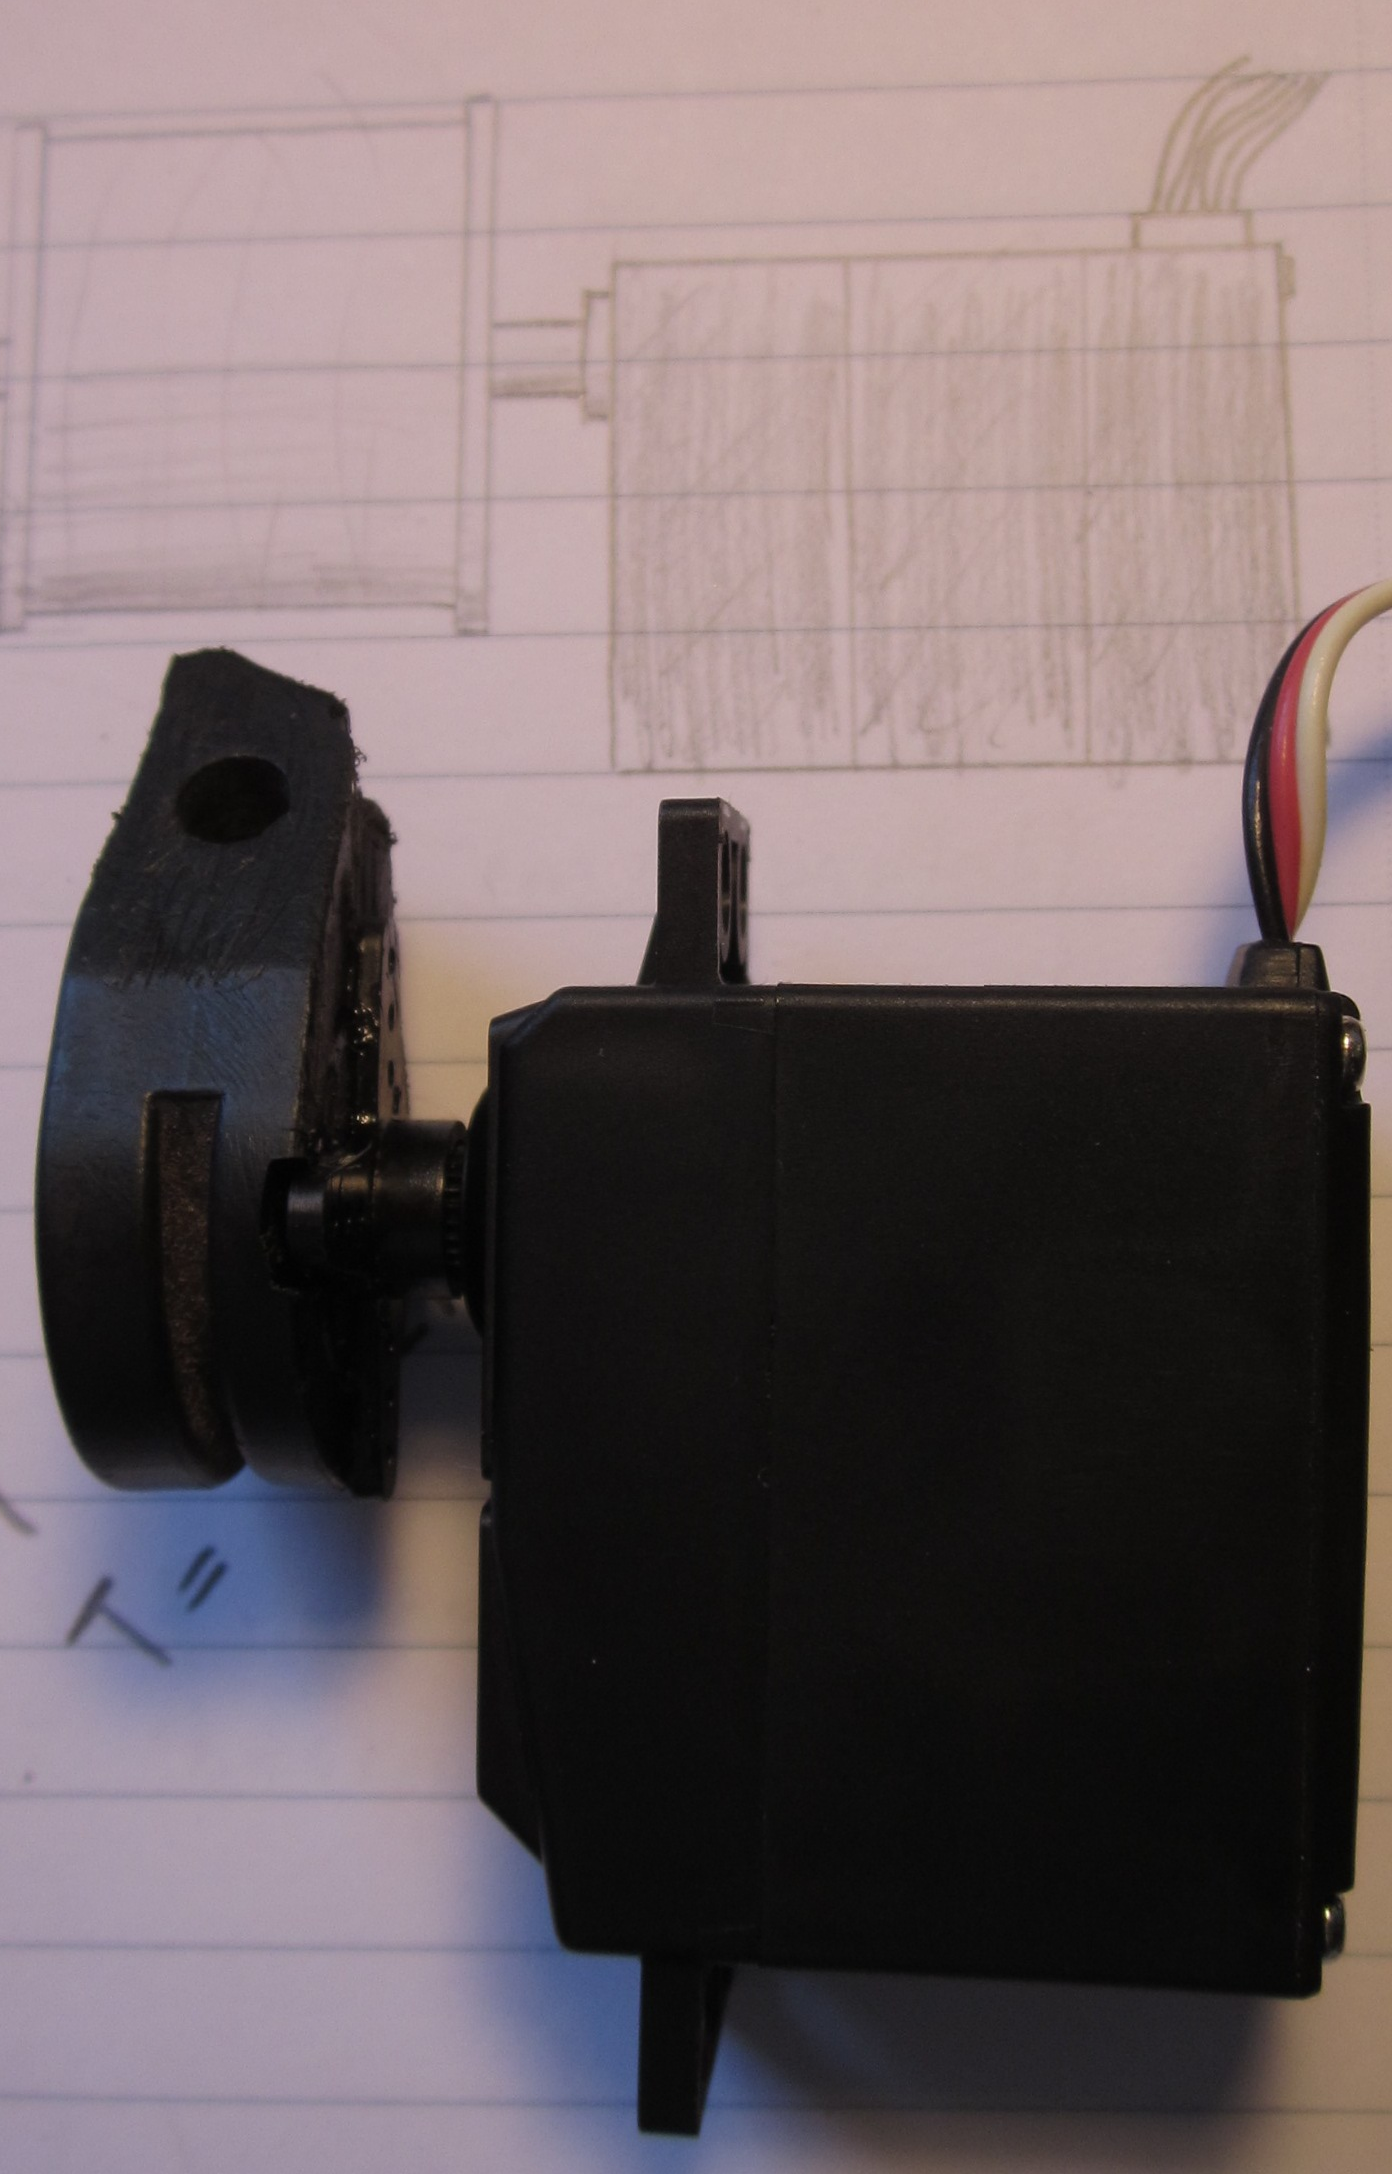
\includegraphics[width=1.9in]{polia3}}
  \caption{Sequência de adaptação do atuador}
  \label{fig:atuador}
\end{figure}


Pequenos servos RC (motores destinados ao mercado de hobbistas) são baratos,
fáceis de encontrar, robustos e seu controle é feito por um sinal PWM. O
servo motor escolhido foi um Futaba S3004, visto na figura \ref{fig:
servo}. O S3004 possui rolamentos de esferas no eixo de saída, e torque de
4.1kg-cm a 6 volts.

\begin{figure}[ht]
 \begin{center}
  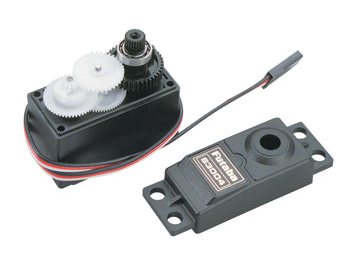
\includegraphics[width=3.2in]{S3004}
 \end{center}
 \caption{Servo Futaba S3004}
 \label{fig: servo}
\end{figure}

Dois complicadores existem na utilização de servos motores\cite{servo}, em
relação a seu comportamento elétrico. O primeiro, como todo componente indutivo,
são os picos de corrente a cada mudança de posição, que podem drenar toda
corrente destinada ao controlador. O segundo complicador é o ruído, tanto gerado
pelo servo nas escovas do motor DC, quanto captado pelo cabo de sinal -- é comum
ver um servo "tremendo" quando em repouso, pois o cabo do sinal atua como uma
antena. Para mitigar estes efeitos a alimentação do servo foi isolada da
alimentação do resto do protótipo. O único cuidado adicional é manter as
referências no mesmo potencial, ou seja, manter o terra dos dois circuitos no
mesmo potencial.

\subsubsection{Display LCD 16x2}
\label{sec:lcd}

Como o sistema propõe uma interface com o usuário, um display LCD foi escolhido
para executar este papel. A principal vantagem deste tipo de display é o baixo
consumo de energia, essencial em sistemas embarcados, devido a independência de
uma fonte de luz própria. O tamanho de 16 caracteres e duas linhas é suficiente
para mostrar as informações de velocidade imediata, a marcha engatada e o valor
da constante de ajuste, planejadas para esta interface.

O display utilizado é um JHD-162a\cite{lcd} de fabricante desconhecido e
facilmente encontrado no mercado, visto na figura \ref{fig:lcd}.
\begin{figure}[ht]
\begin{center}
 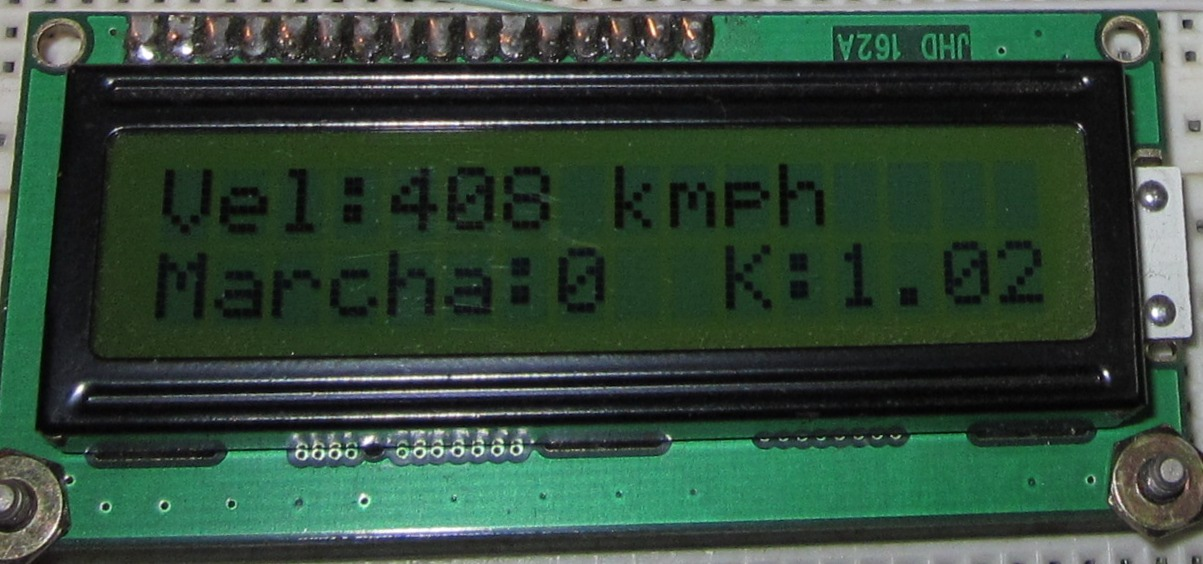
\includegraphics[width=3in]{jhd162a2}
\end{center}
  \caption{Display LCD 16x2}
  \label{fig:lcd}
\end{figure}

A montagem do display não ofereceu nenhum problema, funcionando \textit{out of
the box}, o que é creditado a fartura de boa documentação encontrada na
Internet.

\subsubsection{Reed Switch}
\label{sec:reed}
A definição e uso de elementos sensores foi um dos grandes obstáculos deste
projeto. Estes deveriam ser usados para a leitura de pulsos a cada revolução da
roda e do pedivela, gerando as informações de velocidades, básica ao algoritmo
de controle. As soluções analisadas foram:
\begin{itemize}
 \item Sensor capacitivo
 \item Sensor indutivo
 \item \textit{Reed switch}
 \item Sensor de efeito HALL
\end{itemize}
Os principais critérios de escolha, que permearam o projeto desde sua concepção,
foram simplicidade e custo. O escolhido foi o  \textit{reed switch}, que
oferece uma enorme margem de vantagem nos critérios escolhidos.

Um problema grave dos \textit{reed switch} é o ruído gerado na
sua operação. Devido ao \textit{bouncing}\cite{reed} o sinal gerado precisa de
um tratamento para que possa ser lido corretamente. Foi considerado realizar o
\textit{debounce} do sinal de duas formas: via software; ou via hardware. A
primeira foi descartada pois as funções do programa responsáveis pelo
cálculo de velocidade seriam rotinas de interrupção, ou seja, eles devem ter uma
execução muito breve, caso contrário podem afetar a contagem de tempo do
sistema. Uma função de \textit{debounce} em software envolve, inerentemente
algum \textit{delay}.

\begin{figure}[ht]
 \begin{center}
  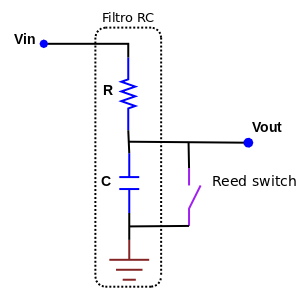
\includegraphics[width=2.8in]{lowpass}
 \end{center}
 \caption{Filtro passa-baixa passivo acoplado ao \textit{reed switch}}
 \label{fig:lowpass}
\end{figure}

A única saída foi mesmo implementar o \textit{debounce} em hardware, utilizando
um filtro passa-baixa passivo, que usa apenas um resistor e um capacitor, de
acordo com o esquema da Figura \ref{fig:lowpass}. O ruído de um \textit{reed
switch} comum está na faixa de 1500Hz a 2000Hz\cite{reed}. É possível estimar a
frequência máxima ($f_{max}$) de ativação dos \textit{reeds} a partir de um
limite de velocidade da roda ($v_{max} = 90 km/h = 25 m/s$):
\begin{equation}
  v = \omega r = 2\pi f r \Rightarrow v_{max} = 2\pi f_{max} r
\end{equation}
O diâmetro da roda com pneu foi medido em d=65cm = 0.65m. Portanto, para
velocidade máxima de 90 km/h:
\begin{equation}
  f_{max} = \frac{\displaystyle v_{max}}{\displaystyle \pi d} =
\frac{\displaystyle 25}{\displaystyle \pi 0.65} = 12.243 Hz
\end{equation}
Tomando a frequência de corte ($f_{c}$) dada pela relação,
\begin{equation}
  f_{c} = \frac{\displaystyle 1}{\displaystyle 2\pi\tau} \text{, onde } \tau =
RC
\end{equation}
igual a frequência máxima ($f_{max}$), diversas combinações de resistores e
capacitores são possíveis. Logo, o script \ref{code:filter} escrito em
linguagem pyhton\cite{python} foi usado para ajudar a dimensionar os
componentes, de acordo com o que foi adquirido (Sec. \ref{custos}) e o que foi
obtido.

\subsubsection{Push buttons}
\label{sec:buttons}
Os \textit{push buttons} têm a função de modificação da constante de ajuste do
sistema, incrementado ou decrementando seu valor. São elementos bastante
simples, que como os \textit{reed switch}, produzem ruído pelo fenômeno de
\textit{bouncing}. Porém como a sua aplicação não é crítica, não houve a
preocupação em tratar o sinal, pois o funcionamento do sistema praticamente não
é prejudicado por estas falhas.
\begin{figure}[ht]
\begin{center}
 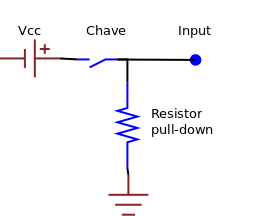
\includegraphics[width=2.5in]{pulldown}
\end{center}
  \caption{Resistor \textit{pull-down}}
  \label{fig:pulldown}
\end{figure}

A única observação feita em relação a montagem dos \textit{push buttons} é a
topologia \textit{pull-down} do resistor, mostrado na figura \ref{fig:pulldown}.
Este dispositivo é usado para limitar a corrente que passa do $V_{cc}$ para o
terra, e para garantir que o nível lógico seja coerente quando a chave conectada
está inativa, ``puxando'' a corrente para o terra. Tipicamente utiliza-se valor
de resistência de 10k$\Omega$, o que foi respeitado na montagem.



\subsubsection{Microcontrolador (MCU)}
\label{sec:mcu}
O microcontrolador utilizado é um ATMega168 20PU do fabricante
Atmel\textsuperscript{\textregistered}. O ATMega168\cite{atmega} é um
microcontrolador de 8 bits com 16K bytes de memória de programa e clock de 20MHz
e arquitetura RISC. O ATMega168 possui diversos periféricos dentre os quais são
de interesse para o projeto:
\begin{itemize}
  \item 6 canais PWM
  \item 23 I/O programáveis (digitais e analógicos)
  \item Interrupção e \textit{wake-up} na borda de subida ou descida de sinal
  \item Interface serial para programação
\end{itemize}

A utilização direta do microcontrolador requer diversos cuidados em relação a
sua alimentação, configuração de pinagem e recursos. Qualquer desenvolvedor de
sistemas embarcados sabe que este tipo de cuidado toma grande quantidade de
tempo e pode ser fonte de infindáveis problemas. Como resolver problemas de
natureza eletrônica e configuração de bits não é o propósito deste trabalho,
foi feita a escolha por uma plataforma de prototipagem que resolve grande parte
deste problemas: o Arduino\cite{arduino}\cite{oxer2009practical}.

O Arduino é uma plataforma de prototipagem \textit{open-source} (hardware e
software) que utiliza microcontroladores Atmel Mega168, Mega328 e Mega1280. Além
dos recursos providos pelo microcontrolador, são embarcados conversor
USB/Serial, tornando desnecessária uma porta serial no PC de desenvolvimento,
\textit{bournes} para conexão dos pinos de I/O, botão de \textit{reset},
cristal oscilador externo e entrada de alimentação. O circuito é capaz
de selecionar automaticamente qual fonte de alimentação utilizar (USB ou fonte
externa).

O modelo de escolhido para este trabalho foi o \textit{Duemilanove}, que
utiliza o microcontrolador ATMega168, e pode ser visto na figura
\ref{fig:duemilanove}.
% FOTO Duemilenove
\begin{figure}[h]
\begin{center}
 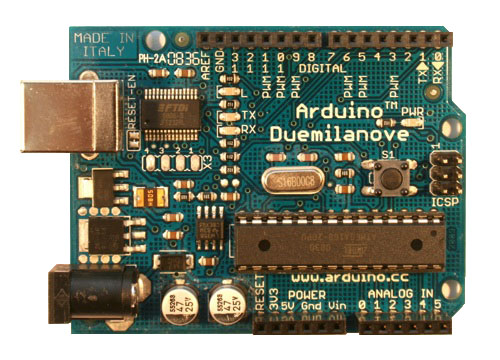
\includegraphics[width=3in]{duemilanove}
\end{center}
  \caption{Arduino Duemilanove}
  \label{fig:duemilanove}
\end{figure}


A linguagem de programação utilizada é o C/C++, sendo que o compilador
utilizado foi o GNU Compiler Collection, o GCC\cite{gcc}. Uma das grandes
vantagem da utilização do GCC é ser multiplataforma, além do fato de ser
software livre. O Arduino provêm uma IDE e bibliotecas para o desenvolvimento
de aplicações, das quais foram utilizadas no projeto as bibliotecas
\textit{Servo} e \textit{LiquidCrystal}, responsáveis pela manipulação de servo
motores e display LCD, respectivamente.


%%%
%
\subsection{Protótipo}
\label{sec:prototipo}
O circuito completo do projeto, conforme esquematizado na figura
\ref{fig:montagem} é apresentado na figura \ref{fig:circuito}.
\begin{figure}[h]
\begin{center}
 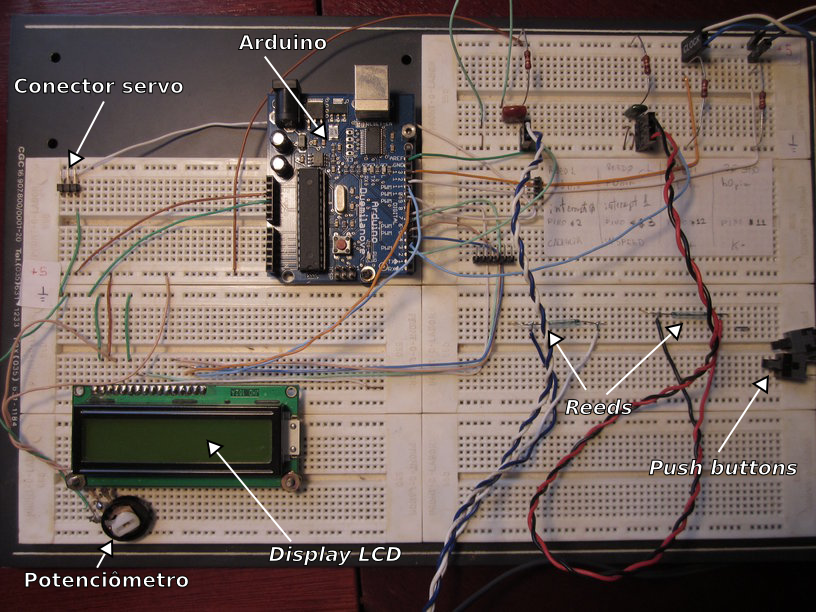
\includegraphics[width=5.5in]{circ_detail}
\end{center}
  \caption{Circuito completo do Projeto}
  \label{fig:circuito}
\end{figure}
O único componente adicional é o potenciômetro, usado para regular o contraste
do display LCD. Destaca-se na metade superior direita os circuitos para
tratamento das entradas (dois filtros passa-baixa e duas montagens de resistor
\textit{pull-down}).

%%%
%
%\pagebreak

\subsection{Algoritmo de controle}
\label{sec:software}
A lógica do programa, elaborada ainda na primeira parte deste trabalho e que se
manteve fiel ao design original é apresentada na figura \ref{fig:fluxograma1} e
descrita a seguir.

\begin{figure}[hb!]
 \begin{center}
  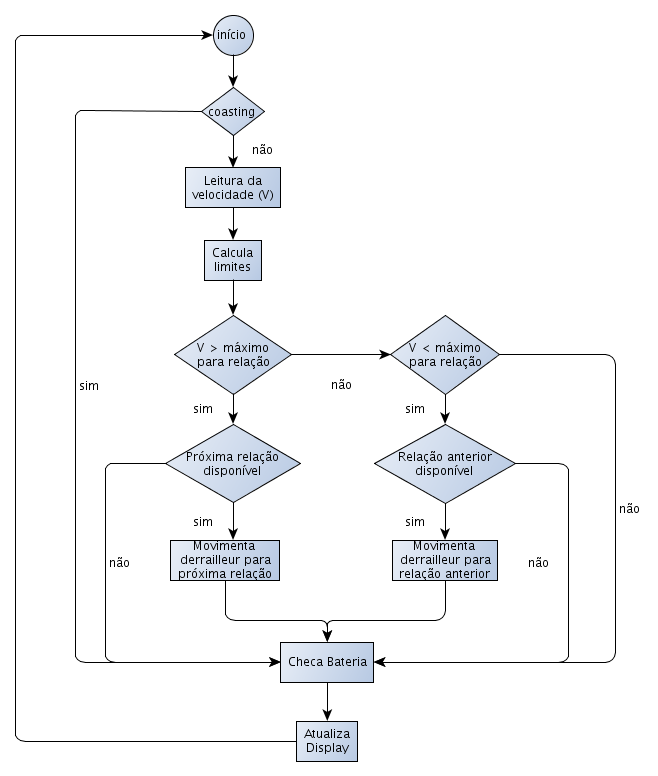
\includegraphics[width=4.65in]{fluxograma1}
 \end{center}
 \caption{Lógica do programa de automação da transmissão}
 \label{fig:fluxograma1}
\end{figure}

\begin{description*}
  \item[Inicio:] início do programa.
  \item[Pedalando:] recebe informação da cadência e se nula, significa que o
  ciclista não está pedalando. Nesse caso, o sistema passa para o teste de
  bateria  e atualização do display. Caso contrário, segue para o passo
  seguinte, de  leitura de velocidade.
  \item[Leitura de velocidade:] armazena a leitura de velocidade instantânea do
  sensor de velocidade da roda traseira.
  \item[Calcula limites:] a partir de uma tabela de limites padrão e do valor da
  constante de velocidade (variável que armazena o valor do multiplicador dos
  limites, para adequação ao estilo de pedalada do ciclista), é calculado o
  limite de velocidade inferior e superior para a marcha presente.
  \item[Velocidade além do limite superior para a relação:] compara leitura de
  velocidade da roda traseira com o calculo do limite superior de velocidade
  para a marcha.
  \item[Velocidade além do limite inferior para a relação:] compara leitura de
  velocidade da roda traseira com o calculo do limite inferior de velocidade
  para a marcha.
  \item[Próxima coroa disponível:] checa se a coroa atual engrenada é a última
  (coroa
  com menos dentes, ou seja, de maior velocidade).
  \item[Coroa anterior disponível:] checa se a coroa atual engrenada é a
  primeira (coroa com mais dentes, ou seja, de maior torque).
  \item[Movimenta \textit{derailleur} para próxima coroa:] caso a velocidade
  seja  maior que o limite superior da coroa atual e exista a próxima coroa, o
  \textit{derailleur}  é movimentado para engatar a coroa seguinte.
  \item[Movimenta \textit{derailleur} para coroa anterior:] caso a velocidade
  seja  menor que o limite inferior da coroa atual e exista a coroa anterior, o
  \textit{derailleur}  é movimentado para engatar a coroa anterior.
  \item[Checa bateria:] testa a carga da bateria e armazena informação. Esta é
  uma etapa muito importante em qualquer dispositivo embarcado, pois é da
  bateria que vem a energia necessária ao funcionamento do sistema.
  \item[Atualiza display:] atualização da interface com informação de velocidade
  instantânea, marcha engatada, e carga da bateria.
\end{description*}

\subsubsection{Implementação}
\label{sec:implemt}

A implementação do algoritmo foi feita criando uma biblioteca para
modelamento das partes físicas e através de uma máquina de  estados. O código
está mostrado nas seções \ref{code:api}, \ref{code:impl} e \ref{code:main}. A
seção \ref{sec:resultados} Teste e Resultados apresenta as adaptações e
detalhes da implementação.


\pagebreak
%%%
%
\section{Testes e Resultados}
\label{sec:resultados}
%TODO teste
%TODO testador lego
%TODO detalhes da implementação
definir cenários de uso, fotos, resultados, ajustes,
detalhes da implementação, iteração...

\pagebreak
%%%
%
\section{Conclusões}
\label{sec:conclusoes}
%TODO concluir Redundância da introdução Dificuldades
\texttt{concluir}

Em tempos de aumento da preocupação com questões ambientais, emissão de
poluentes, humanização das cidades, -- descaracterizadas e transformadas para
servir aos veículos automotores -- a bicicleta aparece como um agente
transformador. Seu apelo a saúde e a ecologia, baixo custo e facilidade de uso
já a promovem ao veículo urbano do futuro, sendo que as diversas iniciativas de
incentivo ao uso de bicicletas comunitárias e/ou públicas ao redor do mundo, e
inclusive em nossa Universidade, estão aí para comprovar esta teoria. 

Muitas extensões podem ser feitas neste projeto, visto que como uma prova de
conceito, é uma implementação muito simplificada. A primeira adição proposta
é adicionar um segundo atuador para ser capaz de manipular o
\textit{derailleur} das coroas dianteiras, podendo utilizar toda a extensão das
marchas disponíveis. Uma forma de incluir esse atuador no algoritmo seria
realizar as trocas nas coroas dianteiras quando a mudança de velocidade for
mais brusca. Isso porque a relação entre as coroas dianteiras é tipicamente
maior quando comparadas a relação entre as coroas do cassete.

Uma segunda sugestão é um sistema de gerenciamento de energia, com baterias e
dínamos de roda, que seriam capazes de manter o sistema rodando apenas com a
própria geração de energia.

A terceira sugestão é a possibilidade de configuração de parâmetros em
\textit{runtime}, além de apenas a constante de ajuste K.

Como quarta, a adição de módulos de memória persistente para
que configurações não sejam perdidas a cada desligamento do sistema.

Finalmente, a quinta e última sugestão é a integração de um acelerômetro
eletrônico, de onde é possível ler a informação de inclinação do terreno. Como
em um automóvel, por vezes é interessante adiar a troca de marcha em subidas (a
"esticada") e postergar na descida.

Por fim e ao cabo, apesar da conclusão sem sucesso, a oportunidade de aplicar a
parte mais interessante de todo o conhecimento acumulado na graduação e bater
de frente em dificuldades da engenharia real foi bastante satisfatória.
Ressalto que o trabalho de graduação está finalizado, e que não pode se dizer o
mesmo para o projeto do câmbio automático para bicicletas.

\begin{figure}[h!]
\begin{center}
 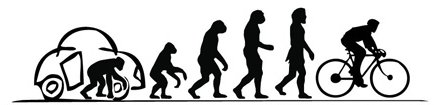
\includegraphics[width=4in]{evo}
\end{center}
\end{figure}


\pagebreak
%%%
%
\section{Anexos}
\label{sec:anexos}

%%%
%

%%%
%
\subsection{Custos do Projeto}
\label{custos}
Os custos dos materiais utilizados foram relativamente baixos. O
reaproveitamento de componentes previamente adquiridos, e principalmente, o
baixo custo dos componentes envolvidos possibilitaram minimizar esta soma. A
Tabela \ref{tab:custos} a seguir computa os componentes e ferramentas.
{
\newcommand{\mc}[3]{\multicolumn{#1}{#2}{#3}}
\begin{table}[ht]
\begin{center}
\caption{Custos do projeto}
\label{tab:custos}
\begin{tabular}{lc}
\mc{1}{c}{\textbf{Material}} & \textbf{Preço (R\$)}\\\hline
Movimento central & R\$ 12,00\\
Display LCD 16x2 & R\$ 20,00\\
Arduino Duemilenove & R\$ 40,00\\
Servo Futaba s3004 & R\$ 12,00\\
Ferro de solda 100W & R\$ 18,00\\
\textit{Reed switch} (5x) & R\$ 3,45\\
Resistores 10k (6x) & R\$ 0,78\\\hline
\textbf{Total} & \textbf{R\$ 106,23}\\\hline
\end{tabular}
\end{center}
\end{table}
}



%%%
%
\subsection{Código Fonte}
\label{codigo}

\subsubsection{API da Biblioteca \textit{BikeTransmission}}
\label{code:api}
\textit{BikeTransmission.h}:
\lstinputlisting{../BikeTransmission/BikeTransmission.h}

\subsubsection{Implementação da Biblioteca \textit{BikeTransmission}}
\label{code:impl}
\textit{BikeTransmission.cpp}:
\lstinputlisting{../BikeTransmission/BikeTransmission.cpp}

\subsubsection{Programa principal}
\label{code:main}
\textit{principal.pde}
\lstinputlisting{../principal/principal.pde}

%%
%
\lstset{frame=single,
    language=Python,
    basicstyle=\ttfamily\small,
    otherkeywords={=, +, [, ], (, ), \{, \}, :},
    keywordstyle=\color{blue},
    stringstyle=\color{red},
    showstringspaces=false,
    emph={class, pass, in, for, while, if, is, elif, else, not, and, or,
    def, print, exec, break, continue, return},
    emphstyle=\color{black}\bfseries,
    emph={[2]True, False, None, self},
    emphstyle=[2]\color{key},
    emph={[3]from, import, as},
    emphstyle=[3]\color{blue},
    upquote=true,
    morecomment=[s]{"""}{"""},
    commentstyle=\color[RGB]{105,105,105}\slshape,
    basicstyle=\tiny,
}
\subsubsection{Cálculo de Relação entre marchas}
\label{code:ratios}
\textit{ratios.py}
\lstinputlisting{../ratios.py}

\subsubsection{Cálculo de Filtro RC}
\label{code:filter}
\textit{capacitance\_n\_resistance.py}
\lstinputlisting{../capacitance_n_resistance_calc.py}




\pagebreak
%%%
%
% bibliografia precisa ser explicitamente adicionada ao sumário:
\addcontentsline{toc}{section}{Referências}
\bibliographystyle{plain}
\bibliography{report}

\end{document}
